% This work is licensed under the Creative Commons Attribution-NonCommercial 4.0 International License.
% To view a copy of this license, visit http://creativecommons.org/licenses/by-nc/4.0/
% or send a letter to Creative Commons, PO Box 1866, Mountain View, CA 94042, USA.

% !TEX TS-program = xelatex

\documentclass[../Main/chem331-notes.tex]{subfiles}
\begin{document}

\setcounter{section}{3}

\section{The Schr\"{o}dinger equation}
\subsection{The time-dependent Schr\"{o}dinger equation}
Recall Newton's second law of motion $\mathbf{F} = m \mathbf{a}$, where $\mathbf{F}$ is the force on an object of mass $m$ and $\mathbf{a}$ is the acceleration. Rewriting the acceleration in terms of the position $\mathbf{x}$ it is clear that Newton's second law is a differential equation
\begin{equation}
\mathbf{F} = m \mathbf{a} = m \frac{d \mathbf{v}(t)}{dt} = m \frac{d^2 \mathbf{r}(t)}{dt^2}.
\end{equation}
In quantum mechanics particles behave like waves. So the fundamental equation that governs them is somewhat different from Newton's second law.
Instead of describing the position of a particle as a function of time, in quantum mechanics we have an equation that describes the evolution of a particle probability amplitude, the so-called \textbf{wave function}.
For a particle in one dimension the wave function is a \textbf{complex} function $\Psi(x,t)$ that depends both on the position of a particle ($x$) and time ($t$).
 The equation that governs the evolution of the wave function is the time-dependent \textbf{Schr\"{o}dinger equation}\mnote{After physicist Erwin Schr\"{o}dinger (Austria, 1887--1961).}
\marginpar{
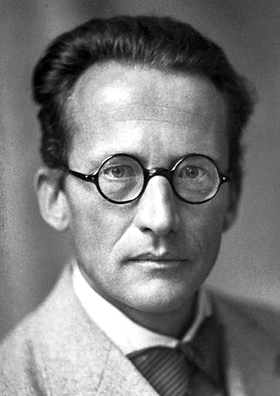
\includegraphics[width=1.5in]{../Figures/02_Erwin_Schrodinger.jpg}
\captionof{figure}{Erwin Schr\"{o}dinger.}
}
\begin{iequation}
i\hbar \frac{\partial \Psi(x,t)}{\partial t} = \hat{H} \Psi(x,t)
\end{iequation}
There are several important elements in the time-dependent Schr\"{o}dinger equation
\begin{ibox}
\begin{myitems}
\item The \textbf{wave function} [$\Psi(x,t)$]. It contains all the information that we can know about a physical system.
\item The \textbf{Hamiltonian operator} [$\hat{H}$]. Operators are mathematical objects that perform operations of function. Given an operator $\hat{O}$, when we apply it to a function $f(x)$ it returns another function $g(x)$, $\hat{O}f(x) = g(x)$.
\item The \textbf{imaginary unit} [$i$]. 
\item The \textbf{reduced Planck constan} [$\hbar = h / 2\pi$, pronounced ``h-bar''].
\end{myitems}
\end{ibox}

\subsection{The wave function and its interpretation}
In quantum mechanics we cannot know the exact position of a particle. Instead we can ask: What is the probability that a particle is at position $x$? This information is contained in the probability density, $\rho(x,t)$, which is given by the square modulus of the wave function
\begin{iequation}
\rho(x,t) = |\Psi(x,t)|^2 = \Psi(x,t)^* \Psi(x,t) = \text{probability density at position $x$ and time $t$},
\end{iequation}
where the asterisk indicates the complex conjugate.
The probability density multiplied by an infinitesimal volume $dx$
\begin{equation}
\rho(x,t) dx = |\Psi(x,t)|^2 dx
\end{equation}
 gives us the probability of finding a particle in the range $[x,x + dx]$ at time $t$.
 Note that we take the modulus square because \textbf{in general the wave function is a complex function}.\mnote{A quantity like $\rho(x,t)$ can be interpreted as a probability only if it is non-negative, that is, if $\rho(x,t) \geq 0$ for all $x$ and $t$.}
 
The probability of finding a particle in the range $[a,b]$ is given by the integral of the probability density
\begin{equation}
P[a \leq x \leq b](t) = \int_a^b dx \, \rho(x,t) = \int_a^b dx \, |\Psi(x,t)|^2.
\end{equation}
Since the probability of finding a particle over all space must be one, the wave function must satisfy the \textbf{normalization condition}
\begin{iequation}
\int_{-\infty}^{\infty} dx \, |\Psi(x,t)|^2 = 1.
\end{iequation}
When a wave function satisfies the normalization condition we say that it is normalized.

\subsection{The Hamiltonian operator}
The Hamiltonian operator is connected to the total energy of a system.
As in classical physics, where the total energy is the sum of kinetic ($T$) and potential energy ($V$), in quantum mechanics the Hamiltonian may be written as
\begin{iequation}
\hat{H} = \hat{T} + \hat{V},
\end{iequation}
where $\hat{T}$ is the kinetic energy operator
\begin{equation}
\hat{T} = - \frac{\hbar^2}{2 m} \frac{\partial^2}{\partial x^2},
\end{equation}
and $\hat{V}$ is the potential energy operator\mnote{In general, the potential could also depend on time $t$, that is, we should write $V(x,t)$. This is the case when we study how a quantum system interacts with a pulse of light. In this case, the potential has a term that accounts for the light pulse and that depends on $t$.}
\begin{equation}
\hat{V} = V(x).
\end{equation}
These operators are very different!
The kinetic energy operator takes the second derivative of a function and multiplies it by a constant, while the potential energy operator is just the classical potential energy function.
Note also that the kinetic energy operator should be accepted as a \textbf{fact of life} (FOL).\mnote{That is, something unpleasant that cannot be avoided.}
Its mathematical expression can be justified but not proven, so it should be taken as a postulate of quantum mechanics.
We will encounter several others FOLs in this course, so get used to this idea.

To summarize, the Hamiltonian for a particle of mass $m$ moving in one dimension is given by
\begin{iequation}
\hat{H} =  - \frac{\hbar^2}{2 m} \frac{\partial^2}{\partial x^2} + V(x).
\end{iequation}


\subsection{The time-independent Schr\"{o}dinger equation}
The time-dependent Schr\"{o}dinger equation tells us how the wave function of a system changes with time.
However, when the potential experienced by a particle does not depend on time, there are solutions of the Schr\"{o}dinger equation that are stationary. These states have physical properties that are constant in time.\mnote{The analogy with classical physics is finding solutions of Newton's equation for which the position of an object is fixed.}
To find stationary states we may try to solve the Schr\"{o}dinger equation using a wave function ansatz\mnote{A German word that stands for ``an assumption about the form of an unknown function which is made in order to facilitate solution of an equation or other problem''.} in which the we write the wave function as the product of two functions $\psi(x)$ and $f(t)$ that depend each on only one variable
\begin{equation}
\Psi(x,t) = \psi(x) f(t)
\end{equation}
If we plug this equation in the time-dependent Schr\"{o}dinger equation we get
\begin{equation}
i\hbar \frac{\partial \psi(x) f(t)}{\partial t} = \hat{H}\psi(x) f(t),
\end{equation}
and rearranging terms we find
\begin{equation}
i\hbar \frac{1}{f(t)}\frac{\partial f(t)}{\partial t} = \frac{\hat{H}\psi(x)}{\psi(x)}.
\end{equation}
Note that the the r.h.s. and l.h.s. of this equation are functions of two independent variables.
So the only way this equation is satisfied is if both sides are equal to a constant, which we well indicated with $E$.
Then we obtain two independent equations. From the l.h.s. we can derive an equation for the function of $t$
\begin{equation}
\label{eq:02:f_equation}
i\hbar \frac{\partial f(t)}{\partial t} = E f(t).
\end{equation}
The solution of this differential equation is
\begin{equation}
\label{eq:02:f_solution}
f(t) = f(t = 0) e^{-i E t / \hbar},
\end{equation}
where $f(t = 0)$ is the value of the function $f(t)$ at $t=0$.
The quantity $e^{-i E t / \hbar}$ is a \textbf{phase factor}, a complex number of absolute value 1.
\begin{exercise}
Show that Eq.~\eqref{eq:02:f_solution} is a solution of Eq.~\eqref{eq:02:f_equation}.
\end{exercise}


From the r.h.s. we obtain an equation for the function of $x$, which is commonly known as the \textbf{time-independent} Schr\"{o}dinger equation
\begin{iequation}
\hat{H}\psi(x) = E \psi(x).
\end{iequation}
This is an eigenvalue equation. $E$ and $\psi(x)$ are called the eigenvalue and eigenfunction of $\hat{H}$, respectively.
Putting all together, we find that the wave function is given by
\begin{equation}
\label{eq:02:factorize_solution}
\Psi(x,t) = f(0) e^{-i E t / \hbar} \psi(x).
\end{equation}
The probability density for this wave function is independent of time
\begin{equation}
|\Psi(x,t)|^2 =  |f(0)|^2 |\psi(x)|^2,
\end{equation}
so Eq.~\eqref{eq:02:factorize_solution} is indeed a stationary wave function.
%\begin{equation}
%\int dx \, \Psi(x,t)^* \Psi(x,t) =  |f(0)|^2 \int dx \,   \left[e^{-i E t / \hbar} \psi(x)\right]^* e^{-i E t / \hbar} \psi(x)
%\end{equation}

We will call the eigenfunctions of the time-independent Schr\"{o}dinger equation \textbf{stationary wave functions}, or simply, wave functions.
For now on we will be mostly concerned with stationary wave functions but we will revisit time-dependent wave functions when we consider the interaction of light with matter.

\subsection{Physical vs. non-physical wave functions}
Not all solutions of the time-independent Schr\"{o}dinger equation are acceptable.
There are three conditions that a function must satisfy to be considered a stationary wave function of a real physical system
\begin{ibox}
\begin{myitems}
\item $\psi(x)$ must be a continuous function of $x$.
\item $\psi(x)$ must be a square-integrable function, that is,
\begin{equation}
\int_{-\infty}^{\infty} dx \, |\psi(x)|^2 < \infty.
\end{equation}
\item $\psi(x)$ must be single valued.
\end{myitems}
\end{ibox}

\subsection{Wave functions and phase factors}
In addition we have to establish one more requirement.
When we solve the time-independent Schr\"{o}dinger equation we have to choose the sign of the solution.
For example, we may find that $\psi(x) = \sin(x)$ is an eigenfunction of the Hamiltonian. In this case any other solution of this form
\begin{equation}
\psi(x) = e^{i\theta} \sin(x),
\end{equation}
where $\theta$ is any real number,  is also acceptable and equivalent to $\psi(x) = \sin(x)$.
The quantity $e^{i\theta}$ is called a phase factor and it is a complex number with modulus equal to one.
Why are these more complex wave functions are equivalent to $\psi(x) = \sin(x)$?
If we compute the probability density for the wave function $\psi(x) = e^{i\theta} \sin(x)$ we find out that it is equal to
\begin{equation}
|\psi(x)|^2 = e^{-i\theta} \sin(x) e^{i\theta} \sin(x) = \sin^2(x),
\end{equation}
which is identical to the probability density of the simpler wave function $\psi(x) = \sin(x)$.
In other words, we discover that multiplying a wave function times $e^{i\theta}$ does not change its probability density.
Since we can choose any value of $\theta$ we have an infinite number of possible solutions.
However, we have to settle for one of those and by default we will always take $\theta = 0$, which gives $e^{i0} = 1$.
Note that if we set $\theta = \pi$ we get $e^{i\pi} = -1$, which corresponds to the solution $\psi(x) = -\sin(x)$.
If we have chosen the solution $\psi(x) = \sin(x)$ then we need to discard $\psi(x) = -\sin(x)$ because according to quantum mechanics  the two represent the same physical states and are therefore equivalent.

\end{document}